% questions.tex —— 2005 年·全国卷Ⅱ·理科 · 题目内容片段（无答案）
% 由 tools/generate_projects.py 依来源总账自 2005/2005_数学真题_全国2理_试题.md 生成，勿手改（改源 MD 后重跑）


\gkpart{数学}

\begin{gktip}
\textbf{来源说明}：本题面依据固定源 PDF 两页 A3 题面逐题转录，原卷印刷页码 252–253。固定源不附答案，答案和解析均由本库独立复算。

\textbf{图形说明}：第 20 题的原卷图形关系重绘为 TikZ/PGFPlots 矢量图。图形标记所指的 PNG 不随仓库保存。
\end{gktip}

\gkpart{一、选择题}

\begin{question}
\gkti{1}函数 $f(x)=|\sin x+\cos x|$ 的最小正周期是\mbox{（　　）}

（A）$\dfrac{\pi}{4}$\quad（B）$\dfrac{\pi}{2}$\quad（C）$\pi$\quad（D）$2\pi$

\end{question}
\begin{question}
\gkti{2}正方体 $ABCD-A_1B_1C_1D_1$ 中，$P\text{、}Q\text{、}R$ 分别是 $AB\text{、}AD\text{、}B_1C_1$ 的中点。那么，正方体的过 $P\text{、}Q\text{、}R$ 的截面图形是\mbox{（　　）}

（A）三角形\quad（B）四边形\quad（C）五边形\quad（D）六边形

\end{question}
\begin{question}
\gkti{3}函数 $y=\sqrt[3]{x^2}-1\ (x\leqslant0)$ 的反函数是\mbox{（　　）}

（A）$y=\sqrt{(x+1)^3}\ (x\geqslant-1)$\quad（B）$y=-\sqrt{(x+1)^3}\ (x\geqslant-1)$

（C）$y=\sqrt{(x+1)^3}\ (x\geqslant0)$\quad（D）$y=-\sqrt{(x+1)^3}\ (x\geqslant0)$

\end{question}
\begin{question}
\gkti{4}已知函数 $y=\tan\omega x$ 在 $\left(-\dfrac{\pi}{2},\dfrac{\pi}{2}\right)$ 内是减函数，则\mbox{（　　）}

（A）$0<\omega\leqslant1$\quad（B）$-1\leqslant\omega<0$\quad（C）$\omega\geqslant1$\quad（D）$\omega\leqslant-1$

\end{question}
\begin{question}
\gkti{5}设 $a\text{、}b\text{、}c\text{、}d\in\mathbb R$，若 $\dfrac{a+bi}{c+di}$ 为实数，则\mbox{（　　）}

（A）$bc+ad\ne0$\quad（B）$bc-ad\ne0$\quad（C）$bc-ad=0$\quad（D）$bc+ad=0$

\end{question}
\begin{question}
\gkti{6}已知双曲线 $\dfrac{x^2}{6}-\dfrac{y^2}{3}=1$ 的焦点为 $F_1\text{、}F_2$，点 $M$ 在双曲线上且 $MF_1\perp x$ 轴，则 $F_1$ 到直线 $F_2M$ 的距离为\mbox{（　　）}

（A）$\dfrac{3\sqrt6}{5}$\quad（B）$\dfrac{5\sqrt6}{6}$\quad（C）$\dfrac65$\quad（D）$\dfrac56$

\end{question}
\begin{question}
\gkti{7}锐角三角形的内角 $A\text{、}B$ 满足 $\tan A-\dfrac1{\sin2A}=\tan B$，则有\mbox{（　　）}

（A）$\sin2A-\cos B=0$\quad（B）$\sin2A+\cos B=0$\quad（C）$\sin2A-\sin B=0$\quad（D）$\sin2A+\sin B=0$

\end{question}
\begin{question}
\gkti{8}已知点 $A(\sqrt3,1)$、$B(0,0)$、$C(\sqrt3,0)$。设 $\angle BAC$ 的平分线 $AE$ 与 $BC$ 相交于 $E$，那么有 $\overrightarrow{BC}=\lambda\overrightarrow{CE}$，其中 $\lambda$ 等于\mbox{（　　）}

（A）$2$\quad（B）$\dfrac12$\quad（C）$-3$\quad（D）$-\dfrac13$

\end{question}
\begin{question}
\gkti{9}已知集合 $M=\{x\mid x^2-3x-28\leqslant0\}$，$N=\{x\mid x^2-x-6>0\}$，则 $M\cap N$ 为\mbox{（　　）}

（A）$\{x\mid-4\leqslant x<-2\text{ \text{或} }3<x\leqslant7\}$\quad（B）$\{x\mid-4<x\leqslant-2\text{ \text{或} }3\leqslant x<7\}$

（C）$\{x\mid x\leqslant-2\text{ \text{或} }x>3\}$\quad（D）$\{x\mid x<-2\text{ \text{或} }x\geqslant3\}$

\end{question}
\begin{question}
\gkti{10}点 $P$ 在平面上作匀速直线运动，速度向量 $\vec v=(4,-3)$（即点 $P$ 的运动方向与 $\vec v$ 相同，且每秒移动的距离为 $|\vec v|$ 个单位）。设开始时点 $P$ 的坐标为 $(-10,10)$，则 $5$ 秒后点 $P$ 的坐标为\mbox{（　　）}

（A）$(-2,4)$\quad（B）$(-30,25)$\quad（C）$(10,-5)$\quad（D）$(5,-10)$

\end{question}
\begin{question}
\gkti{11}如果 $a_1,a_2,\ldots,a_8$ 为各项都大于零的等差数列，公差 $d\ne0$，则\mbox{（　　）}

（A）$a_1a_8>a_4a_5$\quad（B）$a_1a_8<a_4a_5$\quad（C）$a_1+a_8>a_4+a_5$\quad（D）$a_1a_8=a_4a_5$

\end{question}
\begin{question}
\gkti{12}将半径都为 $1$ 的 $4$ 个铅球完全装入形状为正四面体的容器里，这个正四面体的高最小值为\mbox{（　　）}

（A）$\dfrac{\sqrt3+2\sqrt6}{3}$\quad（B）$2+\dfrac{2\sqrt6}{3}$\quad（C）$4+\dfrac{2\sqrt6}{3}$\quad（D）$\dfrac{4\sqrt3+2\sqrt6}{3}$

\end{question}
\gkpart{二、填空题}

\begin{question}
\gkti{13}圆心为 $(1,2)$ 且与直线 $5x-12y-7=0$ 相切的圆的方程为\gkblank{}。

\end{question}
\begin{question}
\gkti{14}设 $\alpha$ 为第四象限的角，若 $\dfrac{\sin3\alpha}{\sin\alpha}=\dfrac{13}{5}$，则 $\tan2\alpha=$\gkblank{}。

\end{question}
\begin{question}
\gkti{15}在由数字 $0,1,2,3,4,5$ 所组成的没有重复数字的四位数中，不能被 $5$ 整除的数共有\gkblank{}个。

\end{question}
\begin{question}
\gkti{16}下面是关于三棱锥的四个命题：

① 底面是等边三角形，侧面与底面所成的二面角都相等的三棱锥是正三棱锥；

② 底面是等边三角形，侧面都是等腰三角形的三棱锥是正三棱锥；

③ 底面是等边三角形，侧面的面积都相等的三棱锥是正三棱锥；

④ 侧棱与底面所成的角都相等，且侧面与底面所成的二面角都相等的三棱锥是正三棱锥。

其中，真命题的编号是\gkblank{}。（写出所有真命题的编号）

\end{question}
\gkpart{三、解答题}

\begin{question}
\gkti{17}设函数 $f(x)=2^{|x+1|-|x-1|}$，求使 $f(x)\geqslant2\sqrt2$ 的 $x$ 的取值范围。

\end{question}
\begin{question}
\gkti{18}已知 $\{a_n\}$ 是各项均为正数的等差数列，$\lg a_1\text{、}\lg a_2\text{、}\lg a_4$ 成等差数列。又

\nopagebreak[4]
\[
b_n=\frac1{a_{2^n}},\qquad n=1,2,3,\ldots\text{。}
\]

（1） 证明 $\{b_n\}$ 为等比数列；

（2） 如果无穷等比数列 $\{b_n\}$ 各项的和 $S=\dfrac13$，求数列 $\{a_n\}$ 的首项 $a_1$ 和公差 $d$。

注：无穷数列各项的和即当 $n\to\infty$ 时数列前 $n$ 项和的极限。

\end{question}
\begin{question}
\gkti{19}甲、乙两队进行一场排球比赛。根据以往经验，单局比赛甲队胜乙队的概率为 $0.6$，本场比赛采用五局三胜制，即先胜三局的队获胜，比赛结束，设各局比赛相互间没有影响。令 $\xi$ 为本场比赛的局数，求 $\xi$ 的概率分布和数学期望。（精确到 $0.0001$）

\Needspace{0.4\textheight}
\end{question}
\begin{question}
\gkti{20}如图，四棱锥 $P-ABCD$ 中，底面 $ABCD$ 为矩形，$PD\perp$ 底面 $ABCD$，$AD=PD$，$E\text{、}F$ 分别为 $CD\text{、}PB$ 的中点。
\nopagebreak[4]
\begin{center}% 2005 年全国卷Ⅱ理科第 20 题：直棱锥
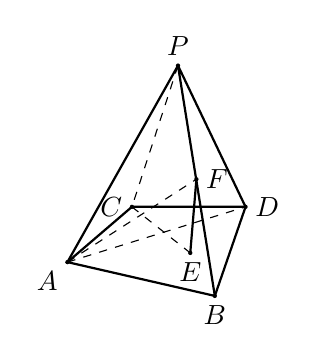
\begin{tikzpicture}[>=stealth,scale=0.78]
  \coordinate (A) at (0,0); \coordinate (B) at (2.4,-0.55);
  \coordinate (C) at (1.05,0.9); \coordinate (D) at (2.9,0.9);
  \coordinate (P) at (1.8,3.2); \coordinate (E) at (2.0,0.15);
  \coordinate (F) at (2.1,1.35);
  \draw[thick] (A)--(B)--(D)--(C)--cycle;
  \draw[thick] (P)--(A) (P)--(B) (P)--(D);
  \draw[dashed] (P)--(C) (A)--(D) (C)--(D);
  \draw[thick] (E)--(F);
  \draw[dashed] (A)--(F) (C)--(E);
  \fill (P) circle (1pt) node[above] {$P$};
  \fill (A) circle (1pt) node[below left] {$A$};
  \fill (B) circle (1pt) node[below] {$B$};
  \fill (C) circle (1pt) node[left] {$C$};
  \fill (D) circle (1pt) node[right] {$D$};
  \fill (E) circle (1pt) node[below] {$E$};
  \fill (F) circle (1pt) node[right] {$F$};
\end{tikzpicture}
\end{center}
\nopagebreak[4]
（1） 求证：$EF\perp$ 平面 $PAB$；

（2） 设 $AB=\sqrt2BC$，求 $AC$ 与平面 $AEF$ 所成的角的大小。

\end{question}
\begin{question}
\gkti{21}$P\text{、}Q\text{、}M\text{、}N$ 四点都在椭圆 $x^2+\dfrac{y^2}{2}=1$ 上，$F$ 为椭圆在 $y$ 轴正半轴上的焦点。已知 $\overrightarrow{PF}$ 与 $\overrightarrow{FQ}$ 共线，$\overrightarrow{MF}$ 与 $\overrightarrow{FN}$ 共线，且 $\overrightarrow{PF}\cdot\overrightarrow{MF}=0$。求四边形 $PMQN$ 的面积的最小值和最大值。

\end{question}
\begin{question}
\gkti{22}已知 $a\geqslant0$，函数 $f(x)=(x^2-2ax)e^x$。

（1） 当 $x$ 为何值时，$f(x)$ 取得最小值？证明你的结论；

（2） 设 $f(x)$ 在 $[-1,1]$ 上是单调函数，求 $a$ 的取值范围。

\end{question}